\chapter{Machine Learining}
\label{ch:MachineLearning}

Before diving into the description of the unsupervised algorithms used for the development of this thesis work presented in \autoref{ch:Unsupervised}, this chapter aim to be an introduction of \emph{Machine Learning} (\gls{ml}) in general.

An early but useful definition of Machine Learning was given by Arthur Samuel in 1959: \quoted{\emph{Machine learning is the field of study that gives computers the ability to learn without being explicitly programmed.}} A more recent definition is the following, from Tom Mitchell: \quoted{\emph{A computer program is said to learn from experience E with respect to some task T and some performance measure P, if its performance on T, as measured by P, improves with experience E.}} \citepage{hands-on-geron2022}{4}

So, in general, the ingredients of \gls{ml} are:
\begin{itemize}
    \item some data linked to some task
    \item a task to be performed
    \item an algorithm that learns how to perform the task on specific data
\end{itemize}

The data are usually preprocessed before giving them to the algorithm. The processed data are called \emph{features}. This is a generic term that refere to the information content of the data.
For example, if the data are recordings of temperatures over time, the features could be the mean, the standard deviation, the minimum, and the maximum of the temperature or, in some cases if the algorithm is able to learn directly from them, the raw data themself.

The tasks can be divided into main categories:
\begin{itemize}
    \item regression: the algorithm is trained to measure the relation between the value of output variables and corresponding values of other input variables;
    \item classification: the algorithm is trained to assign a label to a new instance, based on the training dataset of labeled instances;
    \item clustering: the algorithm is trained to group similar instances together into clusters.
    \item anomaly detection: the algorithm is trained to identify instances that are different from known previous instances.
\end{itemize}

\section{Regression}
\label{sec:Regression}


\subsection{Least Squares}
\label{subsec:LS}

Lets consider a set of $m$ observations of a variable $y \in \mathbb{R}^{n_y}$ (output features) that depends on a variable $x \in \mathbb{R}^{n_x}$ (input features) and a set of $n_f \cdot n_y$ parameters $\theta \in \mathbb{R}^{n_f \times n_y}$.

Supose to know that the output features are linked to the imput features with $n_f$ functions linear in the parameters $\theta$, so that:
\begin{multline*}
    \begin{bmatrix}
        y_1 & y_2 & \dots & y_{n_y} 
    \end{bmatrix}
    =\\
        \begin{bmatrix}
            f_1(x_1, \dots, x_{n_x}) & f_2(x_1, \dots, x_{n_x}) & \dots & f_{n_f}(x_1, \dots, x_{n_x}) \\
        \end{bmatrix}
        \cdot
        \begin{bmatrix}
            \theta_{1,1}  & \dots & \theta_{1,n_y} \\
            \theta_{2,1}  & \dots & \theta_{2,n_y} \\
            \vdots & \ddots & \vdots \\
            \theta_{n_f,1}  & \dots & \theta_{n_f,n_y} \\
        \end{bmatrix}
\end{multline*}

Where all the $f_i$ are any known functions, $y_i$ and $x_i$ are known data and $\theta_{i,j}$ are the parameters to be found.

Considering the $m$ observations, the previous equation can be extended as:

\begin{multline*}
    \begin{bmatrix}
        y_{1,1} & y_{1,2} & \dots & y_{1,n_y} \\
        y_{2,1} & y_{2,2} & \dots & y_{2,n_y} \\
        \vdots & \ddots & \vdots \\
        y_{m,1} & y_{m,2} & \dots & y_{m,n_y} \\
    \end{bmatrix}
    =\\
        \begin{bmatrix}
            f_1(x_{1,1}, \dots, x_{1,n_x}) & \dots & f_{n_f}(x_{1,1}, \dots, x_{1,n_x}) \\
            f_1(x_{2,1}, \dots, x_{2,n_x}) & \dots & f_{n_f}(x_{2,1}, \dots, x_{2,n_x}) \\
            \vdots  & \ddots & \vdots \\
            f_1(x_{m,1}, \dots, x_{m,n_x}) & \dots & f_{n_f}(x_{m,1}, \dots, x_{m,n_x}) \\
        \end{bmatrix}
        \cdot
        \begin{bmatrix}
            \theta_{1,1}  & \dots & \theta_{1,n_y} \\
            \theta_{2,1}  & \dots & \theta_{2,n_y} \\
            \vdots & \ddots & \vdots \\
            \theta_{n_f,1}  & \dots & \theta_{n_f,n_y} \\
        \end{bmatrix}
\end{multline*}


Rewriting the previous equation in a more compact form:

\begin{equation}
    \begin{bmatrix}
        \vect{y}_1 \\
        \vect{y}_2 \\
        \vdots \\
        \vect{y}_m \\
    \end{bmatrix}
    =
    \begin{bmatrix}
        f_1(\vect{x}_1) & f_2(\vect{x}_1) & \dots & f_{n_f}(\vect{x}_1) \\
        f_1(\vect{x}_2) & f_2(\vect{x}_2) & \dots & f_{n_f}(\vect{x}_2) \\
        \vdots & \ddots & \vdots \\
        f_1(\vect{x}_m) & f_2(\vect{x}_m) & \dots & f_{n_f}(\vect{x}_m) \\
    \end{bmatrix}
    \cdot
    \begin{bmatrix}
        \theta_{1,1}  & \dots & \theta_{1,n_y} \\
        \theta_{2,1}  & \dots & \theta_{2,n_y} \\
        \vdots & \ddots & \vdots \\
        \theta_{n_f,1}  & \dots & \theta_{n_f,n_y} \\
    \end{bmatrix}
\end{equation}

That, in the most compact form, becomes:

\begin{equation}
    \vect{Y} = \vect{\Phi}(\vect{X}) \cdot \vect{\Theta}
\end{equation}

In close form, there is a solution $\vect{\Theta_{LS}}$, for estimating the parameters that minimizes the error between the estimated output $\vect{Y_{LS}} = \vect{\Phi(\vect{X})}\vect{\Theta_{LS}}$ and the real output $\vect{Y_{}}$, that is known. Lets see, in an intuitive way:
\begin{eqnarray}
    \vect{Y} &=& \vect{\Phi}(\vect{X}) \cdot \vect{\Theta_{LS}} \\
    \vect{\Phi}(\vect{X})^T\vect{Y} &=& \underbrace{\vect{\Phi}(\vect{X})^T\vect{\Phi}(\vect{X})}_{\text{square}}\cdot \vect{\Theta_{LS}}\\
    (\vect{\Phi}(\vect{X})^T\vect{\Phi}(\vect{X}))^{-1}\vect{\Phi}(\vect{X})^T\vect{Y} &=& \vect{\Theta_{LS}}\\
    \text{pinv}(\vect{\Phi}(\vect{X}))\vect{Y} &=& \vect{\Theta_{LS}} \label{eq:LS}
\end{eqnarray}

In fact, it is known that $\vect{\Theta_{LS}} = \text{pinv}(\vect{\Phi}(\vect{X}))\vect{Y}$ is the solution of the following minimization problem:

\begin{equation}
    \vect{\Theta_{LS}} = \argmin{\vect{\Theta} \in \mathbb{R}^{n_f \times n_y}}{\norm{\vect{Y}-\vect{\Phi}(\vect{X})\vect{\Theta}}_2^2}
\end{equation}

That is why this method is called \emph{Least Squares} (\gls{ls}). It' is proven that if the data $\vect{Y}$ affected my white noise, and the data $\vect{X}$ are known precisely, the solution converges to the real parameters $\vect{\Theta}_{\text{true}}$ when the number of observations $m$ goes to infinity.
\begin{equation}
    \lim_{m \to \infty} \vect{\Theta_{LS}} = \vect{\Theta}_{\text{true}}
\end{equation}

Is this considered machine learning? Yes, even being this just a simple implementation of linear algebra, once programmed in a computer, it qualify as the (simplest) machine learning algorithm because fitting new data does not require any human intervention. Let's see an example. Suppose to have 400 datapoints, shown in \autoref{fig:LinearRegressiondData}, of the variable $x$, $y_1$ and $y_2$ sampled with noise, that we call Fature 1, Feature 2 and Feature 3, respectively. Suppose that it is known that the output features are linked to the input feature with a linear combination of the functions $e^x$, $x^3$, $\cos(x)$, $\sin(x)$ and $\cos^3(x)$, but the parameters $\theta$ are unknown:

\begin{eqnarray}
    y_1 &=& \theta_{1,1} e^x + \theta_{2,1} x^3 + \theta_{3,1} \cos(x) + \theta_{4,1} \sin(x) + \theta_{5,1} \cos^3(x) \\
    y_2 &=& \theta_{1,2} e^x + \theta_{2,2} x^3 + \theta_{3,2} \cos(x) + \theta_{4,2} \sin(x) + \theta_{5,2} \cos^3(x)
\end{eqnarray}

\begin{figure}
    \centering
    \begin{subfigure}{0.49\textwidth}  % <----
        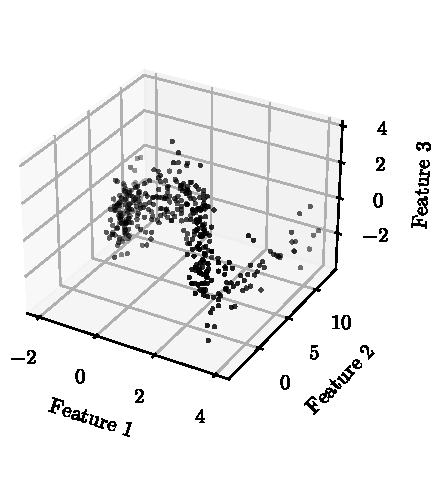
\includegraphics[width=\textwidth]{images/MachineLearning/LinearRegressiondData.pdf}
        \caption{400 datapoints}
        \label{fig:LinearRegressiondData}
    \end{subfigure}
    \begin{subfigure}{0.49\textwidth}  % <----
        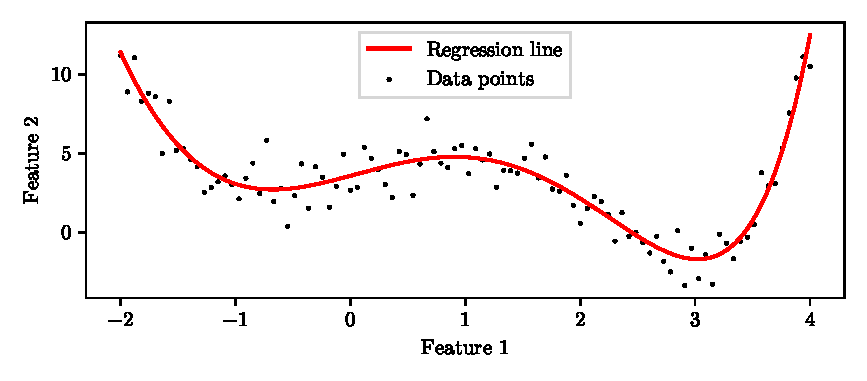
\includegraphics[width=\textwidth]{images/MachineLearning/LinearRegression.pdf}
        \caption{datapoints and the fitted curve}
        \label{fig:LinearRegression}
    \end{subfigure}
    \caption{Least square regression example}
\end{figure}

rearranging in matrix form: 
\begin{equation}
    \underbrace{\begin{bmatrix}
        y_{1,1} & y_{1,2} \\
        y_{2,1} & y_{2,2} \\
        \vdots & \vdots \\
        y_{m,1} & y_{m,2} \\
    \end{bmatrix}}_{\vect{Y}}
    =
    \underbrace{\begin{bmatrix}
        e^{x_1} & x_1^3 & \cos(x_1) & \sin(x_1) & \cos^3(x_1) \\
        e^{x_2} & x_2^3 & \cos(x_2) & \sin(x_2) & \cos^3(x_2) \\
        \vdots & \vdots & \vdots & \vdots & \vdots \\
        e^{x_m} & x_m^3 & \cos(x_m) & \sin(x_m) & \cos^3(x_m) \\
    \end{bmatrix}}_{\vect{\Phi}(\vect{X})}
    \cdot
    \underbrace{\begin{bmatrix}
        \theta_{1,1}  & \theta_{1,2} \\
        \theta_{2,1}  & \theta_{2,2} \\
        \theta_{3,1}  & \theta_{3,2} \\
        \theta_{4,1}  & \theta_{4,2} \\
        \theta_{5,1}  & \theta_{5,2} \\
    \end{bmatrix}}_{\vect{\Theta}}
\end{equation}

applying the \gls{ls} solution from \autoref{eq:LS}, we obtain:
\begin{equation*}
    \vect{\Theta_{LS}} = \text{pinv}(\vect{\Phi}(\vect{X}))\vect{Y} = 
    \begin{bmatrix}
        +1.997 & -0.004 \\
        -1.498 & +0.003 \\
        +1.332 & -0.018 \\
        -0.005 &  +0.999 \\
        -0.032 & +1.035 
    \end{bmatrix}
\end{equation*}

that is quite close to the real parameters used to generate the data:
\begin{equation*}
    \vect{\Theta}_{\text{true}} = 
    \begin{bmatrix}
        +2.0 & +0 \\
        -1.5 & +0 \\
        +1.3 & +0 \\
        +0.0 & +1 \\
        +0.0 & +1 
    \end{bmatrix}
\end{equation*}

Using the estimated parameters, it is possible to estimate the output features for new input features, the regression line is shown in \autoref{fig:LinearRegression}.

\subsubsection{Applicability}
This is an elegant closed form solution for a regression problem, however it has some limitations:
\begin{itemize}
    \item if the noise is not white, or it is present also in the input features, the solution is not guaranteed to converge to the real parameters;
    \item if there are nonlinearity in the parameters (for example $\sin(\theta_{1,1}x)$), the solution is not applicable;
\end{itemize}

\subsection{Gradient Descent \gls{gd}}
To overcome these limitation, another way to estimate the parameters is to use an iterative algorithm that minimize a cost function over the parameters space. The iterations aim to update the parameters in the direction of the steepest descent of the cost function. This can be done even with nonlinearities in the data, and even if the noise is not white, but has the drawback of the risk of getting stuck in a local minimum of the cost function, starting from a random initialization.
Another limitation is the fact that a learning rate $\eta$ has to be defined, that is a parameter that defines how much the parameters are updated at each iteration. If the learning rate is too small, the algorithm will take a lot of time to converge, if it is too large, the algorithm may overshoot the minimum and avoid convergence.

In the previous closed form solution (\autoref{subsec:LS}), the hypotesis function was linear in the parameters $\vect{Y} = \vect{\Phi}(\vect{X})\cdot\vect{\Theta}$, so we can call this prediction $\vect{\hat{y}} = \vect{h}_{\vect{\Theta}}(\vect{x})$.

The cost function to be minimized is usually defined as the mean squared error between the prediction and the real data:
\begin{equation}
    \text{MSE}(\vect{X}, h_{\vect{\Theta}}) = \frac{1}{m}\sum_{i=1}^{m}(\vect{\hat{y}}_i - \vect{y}_i)^2
\end{equation}


The gradient of the cost function, used by all gradient descent algorithms, is defined as:

\begin{equation}
\nabla_{\vect{\Theta}} \text{MSE}(\vect{X}, h_{\vect{\Theta}}) = 
\begin{bmatrix}
    \frac{\partial}{\partial \theta_1} \text{MSE}(\vect{X}, h_{\vect{\Theta}}) \\
    \frac{\partial}{\partial \theta_2} \text{MSE}(\vect{X}, h_{\vect{\Theta}}) \\
    \vdots \\
    \frac{\partial}{\partial \theta_{n_f\times n_y}} \text{MSE}(\vect{X}, h_{\vect{\Theta}}) \\
\end{bmatrix}
\end{equation}

The algorithm than update the parameters at each iteration as:
\begin{equation}
    \vect{\Theta}^{(i+1)} = \vect{\Theta}^{(i)} - \eta \nabla_{\vect{\Theta}} \text{MSE}(\vect{X}, h_{\vect{\Theta}})
\end{equation}


\subsection{Sthocastic Gradient Descent}
\label{subsec:SGD}
The \emph{Stochastic Gradient Descent} (\gls{gd}) is a variant of the \gls{gd} algorithm that compute the gradient only on one instance at each iteration, instead of on the whole dataset. This makes the algorithm much faster, but the cost function will be much more noisy, and theta will not reach a steady value, but instead will oscillate around the minimum. This has the advantage ov being more robust to local minimum entrapment, but the disadvantage of never reaching the minimum. To overcome this, the learning rate $\eta$ can be reduced at each iteration, but this will slow down the convergence.

\begin{figure}
    \centering
    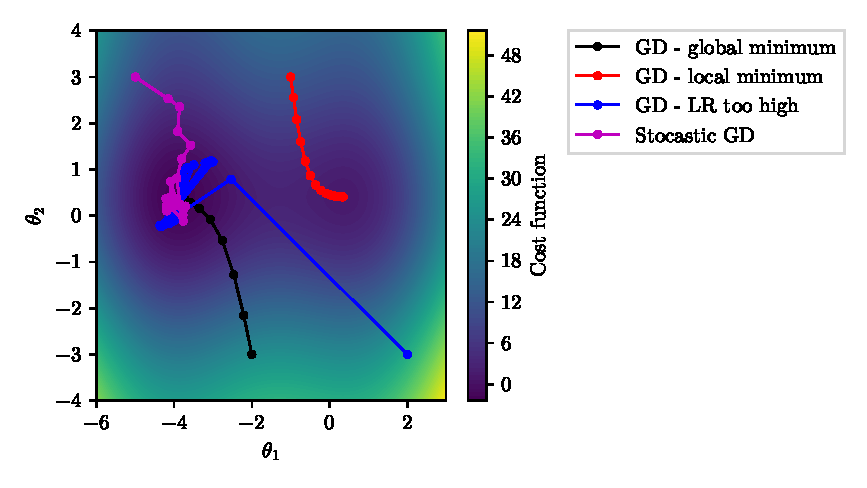
\includegraphics[width=\textwidth]{images/MachineLearning/GradientDescent.pdf}
    \caption{Gradient Descen comparison}
    \label{fig:SGD}
\end{figure}

In the \autoref{fig:SGD} it is visualized graphically what said about Gradient Descent.

\subsection{Avoid overfitting}
\label{subsec:overfitting}
The \gls{gd} algorithm is very powerful, but it can overfit the data. To avoid that, the problem of when to stop the iterations has to be addressed. A common way to do that is to split the dataset into a training set and a validation set. The training set is used to train the algorithm, and the validation set is used to evaluate the performance of the algorithm on new data. The training is stopped when the performance on the validation set starts to degrade, even if the performance on the training set is still improving. This is called \emph{early stopping}.

\begin{figure}
    \centering
    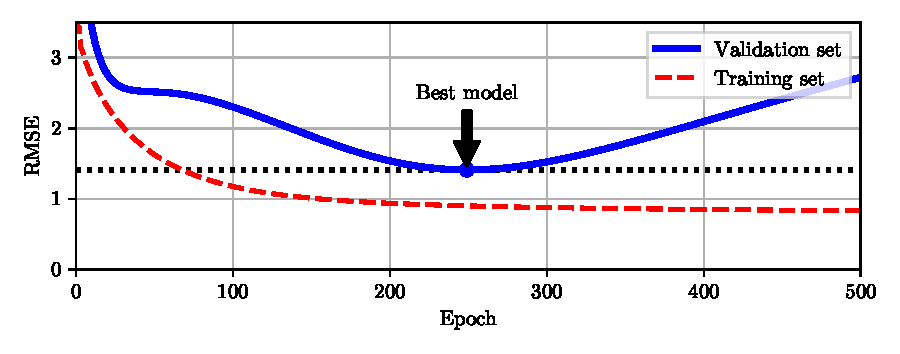
\includegraphics[width=\textwidth]{images/MachineLearning/EarlyStopping.pdf}
    \caption{Overfitting example \citepage{hands-on-geron2022}{162}}
    \label{fig:overfitting}
\end{figure}